\section{Auswertung}
	\label{sec:auswertung}

	F"ur einige Ergebnisse wird im Folgenden ein Mittelwert $\overline{x}$ der gemessenen Gr"o"se $x$ und der entsprechende Fehler $\Delta \overline{x}$ ben"otigt.
	F"ur diese Gr"o"sen gilt bei einem Umfang von $n$ Messwerten

	\begin{eqnarray*}
		\overline{x} & = & \frac{1}{n} \sum_{i=1}^{n}{x_\mathrm{i}} \, , \\
		\Delta \overline{x} & = & \left(\frac{1}{n (n-1)} \sum_{i = 1}^{n}{{\left(x_\mathrm{i} - \overline{x}\right)}^2}\right)^\frac{1}{2} \, .
	\end{eqnarray*}

	\subsection{Verifizierung der Linsen- und Ma"sstabsgleichung}
		\label{subsec:verifizierung}
		Zun"achst sollen die Gleichungen \eqref{abbildungsmassstab} und \eqref{linsengleichung} anhand einer Linse bekannter Brennweite verifiziert werden.
		Dazu werden Bildweite $b$, Bildgr"o"se $B$ und Gegenstandsweite $g$ gemessen.
		Die Gegenstandsgr"o"se wird zu $G = \SI{2.75 (5)}{\centi \meter}$ gemessen und bleibt bei allen folgenden Messungen konstant.

		Die folgende Tabelle enth"alt die Messwerte der Linse mit bekannter Brennweite, sowie die Abbildungsma"sst"abe $V_1 = b/g$ und $V_2 = B/G$ und deren Verh"altnis $V_1/V_2$:

		\begin{table}[!h]
			\begin{center}
				\label{tabelle:bekannt}
				\caption{Messwerte der bekannten Linse}
				\begin{tabular}{|c|c|c|c|c|c|c|}
					\hline 
					$g [\SI{}{\milli \meter}]$ & $b [\SI{}{\milli \meter}]$ & $f$\,[mm] & $B [\SI{}{\milli \meter}]$ & $V_1$ & $V_2$ & $V_1/V_2$ \\
					\hline 
					\hline
					200,5	& 899,5 & 163,56 & 135,0 & 3,854 & 3,964 & 0,972 \\
203,0	& 847,0 & 164,14 & 115,0 & 3,502 & 3,564 & 0,983 \\
206,0	& 794,0 & 163,64 & 109,0 & 3,186 & 3,236 & 0,984 \\
211,0	& 739,0 & 163,78 & 98,0  & 2,837 & 2,909 & 0,975 \\
215,0	& 685,0 & 163,66 & 89,0  & 2,486 & 2,545 & 0,977 \\
221,5	& 628,5 & 163,56 & 80,0  & 2,112 & 2,145 & 0,984 \\
229,5	& 570,5 & 163,17 & 70,0  & 1,703 & 1,745 & 0,976 \\
241,0	& 509,0 & 162,11 & 59,0  & 1,104 & 1,127 & 0,979 \\
259,0	& 441,0 & 163,75 & 48,0  & 4,172 & 4,182 & 0,998 \\
309,0	& 341,0 & 163,95 & 31,0  & 4,486 & 4,909 & 0,914 \\
					\hline 
				\end{tabular}
			\end{center}
		\end{table}

		Zu jedem Wertepaar $(g_\mathrm{i}, b_\mathrm{i})$ kann die Brennweite $f_\mathrm{i}$ bestimmt werden.
		Der Mittelwert $\overline{f}$ wird mit den Herstellerangaben $f_\mathrm{Her}$ verglichen.
		Auf Abweichungen wird in der Diskussion eingegangen.

		Man erh"alt

		\begin{eqnarray*}
			\overline{f} & = & \SI{163.53 (18)}{\milli \meter} \, , \\
			f_\mathrm{Her} & = & \SI{150}{\milli \meter} \, , \\
			\overline{f}/f_\mathrm{Her} & = & \SI{1.09}{} \, .
		\end{eqnarray*}

		Der Mittelwert der Abbildungsverh"altnisse $\overline{V_1/V_2}$ sollte zudem etwa 1 betragen, wenn Gleichung \eqref{abbildungsmassstab} gilt.

		\begin{equation*}
			\overline{V_1/V_2} = \SI{.974}{} \, .
		\end{equation*}

	\clearpage

	\subsection{Brennweite einer unbekannten Linse}
		\label{subsec:unbekannte}
		Die vorherige Messung wird bei einer Linse unbekannter Brennweite wiederholt.
		Folgende Tabelle beinhaltet die Messdaten:

		\begin{table}[!h]
			\begin{center}
				\label{tabelle:unbekannt}
				\caption{Messwerte der unbekannten Linse}
				\begin{tabular}{|c|c|c|c|c|c|c|}
					\hline 
					$g [\SI{}{\milli \meter}]$ & $b [\SI{}{\milli \meter}]$ & $f$\,[mm] & $B [\SI{}{\milli \meter}]$ & $V_1$ & $V_2$ & $V_1/V_2$ \\
					\hline 
					\hline
					201,0 &	299,0 & 120,20 & 42,5  & 1,488 & 1,545 & 0,963 \\
174,0 &	376,0 & 118,95 & 62,0  & 2,161 & 2,255 & 0,958 \\
170,0 &	405,0 & 120,52 & 69,0  & 2,593 & 2,727 & 0,951 \\
167,0 &	433,0 & 120,62 & 75,0  & 3,063 & 3,218 & 0,952 \\
164,0 &	461,0 & 119,84 & 80,0  & 3,560 & 3,764 & 0,946 \\
160,0 &	490,0 & 120,30 & 88,5  & 3,983 & 4,182 & 0,953 \\
157,0 &	518,0 & 121,29 & 95,0  & 3,708 & 4,091 & 0,906 \\
154,0 &	571,0 & 120,48 & 112,5 & 3,299 & 3,455 & 0,955 \\
153,5 &	546,5 & 120,97 & 103,5 & 2,811 & 2,909 & 0,966 \\
150,5 &	599,5 & 119,74 & 115,0 & 2,382 & 2,509 & 0,949 \\
					\hline 
				\end{tabular}
			\end{center}
		\end{table}

		Wie oben folgen aus der Messung die Werte

		\begin{eqnarray*}
			\overline{f} & = & \SI{120.29 (21)}{\milli \meter} \, , \\
			\overline{V_1/V_2} & = & \SI{.950}{} \, .
		\end{eqnarray*}

		Die folgenden Grafiken \ref{fig:graph_bekannt} und \ref{fig:graph_unbekannt} zeigen die Wertepaare $(g_\mathrm{i}, b_\mathrm{i})$ auf den Achsen eines Koordinatensystems eingezeichnet.
		Falls keine Messfehler auftreten, schneiden sich die Geraden im Brennpunkt $(f, f)$.

		Durch Ablesen werden damit die Brennweiten bestimmt zu

		\begin{eqnarray*}
			f_\mathrm{bekannt} & = & \SI{160 (5)}{\milli \meter}\,,\\
			f_\mathrm{unbekannt} & = & \SI{120 (5)}{\milli \meter}\,.
		\end{eqnarray*}

		\begin{figure}[h!]
			\centering
			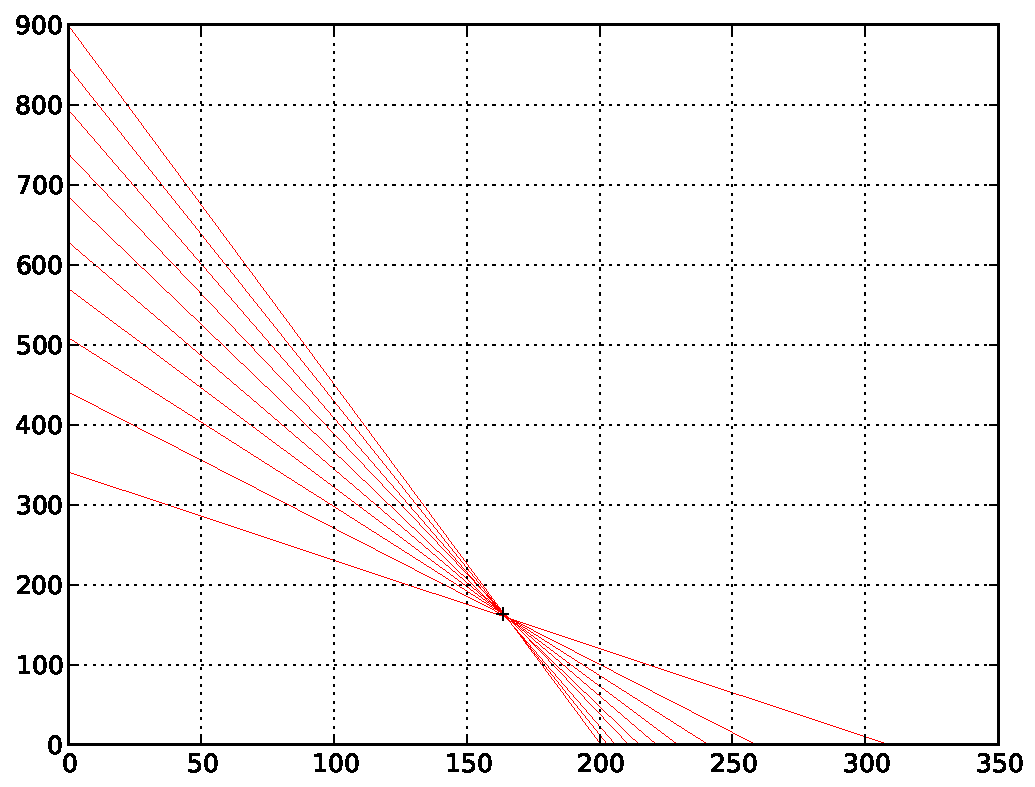
\includegraphics[width = 10cm]{img/graph_bekannt.pdf}
			\caption{Wertepaare $(g_\mathrm{i}, b_\mathrm{i})$ der bekannten Linse auf die x- und y-Achsen eingetragen.}
			\label{fig:graph_bekannt}
		\end{figure}

		\begin{figure}[h!]
			\centering
			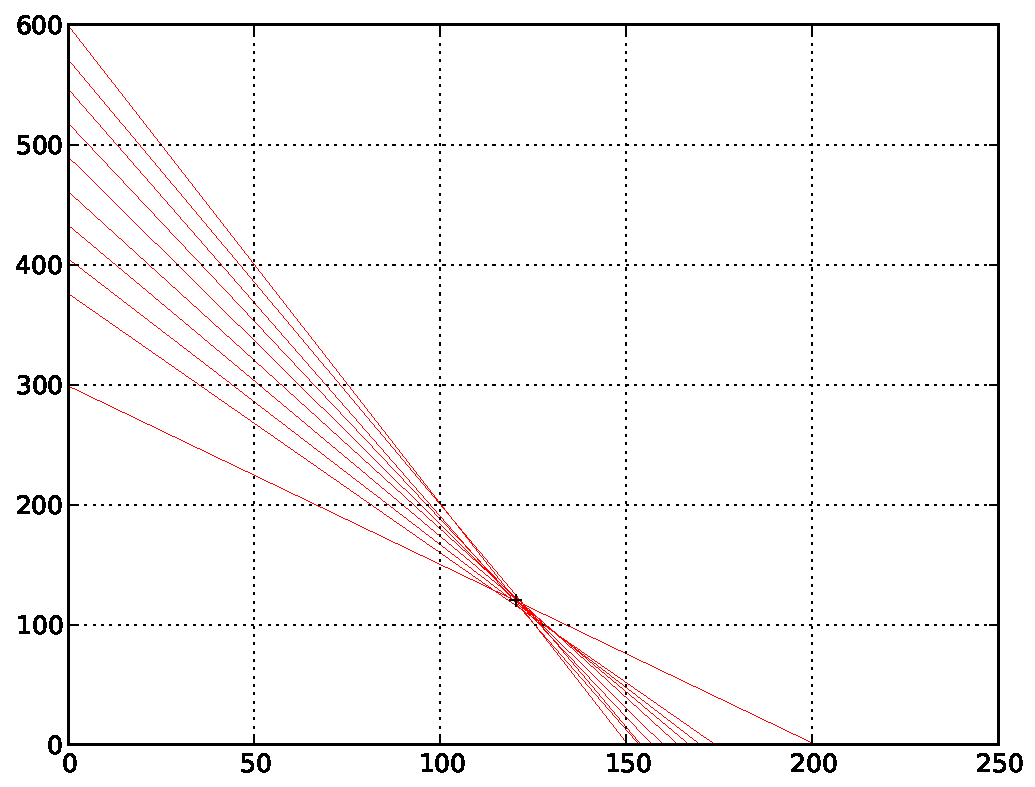
\includegraphics[width = 10cm]{img/graph_unbekannt.pdf}
			\caption{Wertepaare $(g_\mathrm{i}, b_\mathrm{i})$ der unbekannten Linse auf die x- und y-Achsen eingetragen.}
			\label{fig:graph_unbekannt}
		\end{figure}

	\clearpage

	\subsection{Bestimmung der Brennweite einer Linse nach der Methode von Bessel}
		\label{subsec:bessel}
		% F"ur diese Messung werden bei festem Abstand $e$ zwischen Gegenstand und Schirm zwei Wertepaare $(g_{1,\mathrm{i}}, b_{1,\mathrm{i}})$ und $(g_{2,\mathrm{i}}, b_{2,\mathrm{i}})$ gemessen, an denen das Bild scharf erscheint.
		% Zus"atzlich wird das Licht bei f"unf Messungen durch eine rote oder blaue Folie gef"arbt.
		% Hierduch wird der Effekt der chromatischen Abberation untersucht.
		% Tabelle \ref{tabelle:bessel} zeigt die Messdaten f"ur wei"ses, Tabelle \ref{tabelle:farbe} die f"ur gef"arbtes Licht.

		Mit dem Abstand $d$

		\begin{equation*}
			d = |g_1 - b_1| = |g_2 - b_2| \, ,
		\end{equation*}

		zwischen beiden Linsenpositionen gilt die Beziehung

		% Nach Gleichung \eqref{bessel} gilt f"ur die Brennweite $f$:

		\begin{equation}
			f = \frac{e^2 - d^2}{4e} \, .
		\end{equation}

		Folgende Tabellen zeigen die Messwerte f"ur wei"ses, rotes und blaues Licht.

		\begin{table}[!h]
			\begin{center}
				\label{tabelle:bessel}
				\caption{Messwerte der Bild- und Gegenstandsweiten f"ur die Methode nach Bessel mit wei"sem Licht.}
				\begin{tabular}{|c|c|c|c|c|c|c|}
					\hline 
					$g_1 [\SI{}{\milli \meter}]$ & $b_1 [\SI{}{\milli \meter}]$ & $g_2 [\SI{}{\milli \meter}]$ & $b_2 [\SI{}{\milli \meter}]$ & $e [\SI{}{\milli \meter}]$ & $d [\SI{}{\milli \meter}]$ & $f [\SI{}{\milli \meter}]$\\
					\hline 
					\hline
					199,0 & 901,0 & 902,0 & 198,0 & 1000,0 & 571,0 & 168,49 \\
201,5 & 848,5 & 850,0 & 200,0 & 1050,0 & 648,5 & 162,37 \\
208,5 & 741,5 & 742,0 & 208,0 & 1100,0 & 703,0 & 162,68 \\
213,0 & 687,0 & 689,0 & 211,0 &  950,0 & 533,5 & 162,60 \\
219,5 & 630,5 & 631,0 & 219,0 &  900,0 & 476,0 & 162,06 \\
225,0 & 775,0 & 796,0 & 204,0 &  850,0 & 411,5 & 162,70 \\
227,0 & 573,0 & 577,0 & 223,0 &  800,0 & 350,0 & 161,72 \\
238,0 & 512,0 & 513,0 & 237,0 &  750,0 & 275,0 & 162,29 \\
256,0 & 444,0 & 441,0 & 259,0 &  700,0 & 185,0 & 162,78 \\
308,0 & 342,0 & 338,0 & 312,0 &  650,0 &  30,0 & 162,15 \\
					\hline 
				\end{tabular}
			\end{center}
		\end{table}

		\begin{table}[!h]
			\begin{center}
				\label{tabelle:farbe}
				\caption{Messwerte der Bild- und Gegenstandsweiten f"ur die Methode nach Bessel bei blauem und rotem Licht.}
				\begin{tabular}{|c|c|c|c|c|c|c|}
					\hline 
					$g_1 [\SI{}{\milli \meter}]$ & $b_1 [\SI{}{\milli \meter}]$ & $g_2 [\SI{}{\milli \meter}]$ & $b_2 [\SI{}{\milli \meter}]$ & $e [\SI{}{\milli \meter}]$ & $d [\SI{}{\milli \meter}]$ & $f [\SI{}{\milli \meter}]$ \\
					\hline 
					\hline
					\multicolumn{7}{|c|}{rotes Licht}\\
					\hline
					206,0 & 794,0 & 796,0 & 204,0 & 204,5 & 795,5 & 797,0 & 203,0 \\
203,0 & 847,0 & 847,0 & 203,0 & 201,0 & 849,0 & 850,0 & 200,0 \\
202,0 & 898,0 & 809,0 & 291,0 & 200,0 & 900,0 & 901,0 & 199,0 \\
211,0 & 739,0 & 741,0 & 209,0 & 209,0 & 741,0 & 743,0 & 207,0 \\
215,0 & 685,0 & 686,0 & 214,0 & 213,0 & 687,0 & 687,0 & 213,0 \\
					\hline 
				\end{tabular}
			\end{center}
		\end{table}

		\clearpage

		Durch Bildung des Mittelwertes erh"alt man die Brennweiten f"ur wei"ses Licht ($\overline{f}$),
		rotes Licht ($\overline{f_\mathrm{rot}}$) und f"ur blaues Licht ($\overline{f_\mathrm{blau}}$):

		\begin{eqnarray*}
			\overline{f} & = & \SI{162.98 (62)}{\milli \meter} \, , \\
			f_\mathrm{Her} & = & \SI{150}{\milli \meter} \, , \\
			\overline{f}/f_\mathrm{Her} & = & \SI{1.09}{} \, , \\
			\overline{f_\mathrm{rot}} & = & \SI{164.00 (25)}{\milli \meter} \, , \\
			\overline{f_\mathrm{blau}} & = & \SI{162.89 (21)}{\milli \meter} \, , \\
			\overline{f_\mathrm{rot}} - \overline{f_\mathrm{blau}} & = & \SI{1.11 (33)}{\milli \meter}
		\end{eqnarray*}

	\subsection{Bestimmung der Brennweite eines Linsensystems nach der Methode von Abbe}
		\label{subsec:abbe}
		% Bei einem Linsensystem kann die Gegenstands- und Bildweite von verschiedenen Hauptebenen aus gemessen werden.
		% Die Gegenstandsweite $g$ wird dabei von der Hauptebene $H$ und die Bildweite $b$ von der Hauptebene $H'$ gemessen.
		% Von einem beliebigen Punkt $A$ im Linsensystem werden nun die Abst"ande $g'$ und $b'$ zu Gegenstand und Bild gemessen.
		% Dabei gilt

		% \begin{eqnarray}
		% 	g' & = & g + h \, = \, f_1 \left(1 + \frac{1}{V}\right) + h \, , \label{abbe1}\\
		% 	b' & = & b + h' \, = \, f_2 \left(1 + {V}\right) + h' \label{abbe2}\\
		% \end{eqnarray}

		% \begin{center}
		% 	\tiny {(Bei fehlerfreien Messung gilt $f_1 = f_2$)}
		% \end{center}

		% mit

		% \begin{eqnarray*}
		% 	g = g' - h & \Rightarrow & H = A + h \, , \\
		% 	b = b' - h' & \Rightarrow & H' = A + h' \, .\\
		% \end{eqnarray*}

		Eine Lineare Regression der Gleichungen \eqref{abbe1} und \eqref{abbe2} liefert die Brennweite $f$, sowie die Positionen von $h$ und $h'$.
		Die Regression wird mit folgenden Werten durchgef"urt:

		\begin{table}[!h]
			\begin{center}
				\label{tabelle:abbe}
				\caption{Messwerte der Bild- und Gegenstandsweiten zur Hilfsebene $A$ f"ur die Methode nach Abbe.}
				\begin{tabular}{|c|c|c|c|c|}
					\hline 
					$g' [\SI{}{\milli \meter}]$ & $b' [\SI{}{\milli \meter}]$ & $e [\SI{}{\milli \meter}]$ &$B [\SI{}{\milli \meter}]$ & $V$ \\
					\hline 
					\hline
					242,0 & 958,0  & 81,0  & 2,95 \\
251,0 & 899,0  & 73,0  & 2,65 \\
262,0 & 838,0  & 65,0  & 2,36 \\
275,0 & 775,0  & 57,0  & 2,07 \\
291,0 & 709,0  & 50,0  & 1,82 \\
332,0 & 618,0  & 39,0  & 1,42 \\
384,0 & 516,0  & 27,0  & 0,98 \\
235,0 & 1015,0 & 89,0  & 3,24 \\
231,0 & 1069,0 & 95,0  & 3,45 \\
222,0 & 1128,0 & 105,0 & 3,82 \\
					\hline 
				\end{tabular}
			\end{center}
		\end{table}

		Eine lineare Regression mit numpy liefert die Werte

		\begin{eqnarray*}
			f_1 & = & \SI{217.8 (64)}{\milli \meter} \, , \\
			f_2 & = & \SI{217.4 (34)}{\milli \meter} \, , \\
			h & = & \SI{-48.8 (96)}{\milli \meter} \, , \\
			h' & = & \SI{96.7 (123)}{\milli \meter} \, , \\
			\overline{f} = \frac{f_1 + f_2}{2} & = & \SI{217.6 (50)}{\milli \meter}\,.
		\end{eqnarray*}

		\begin{figure}[h!]
			\centering
			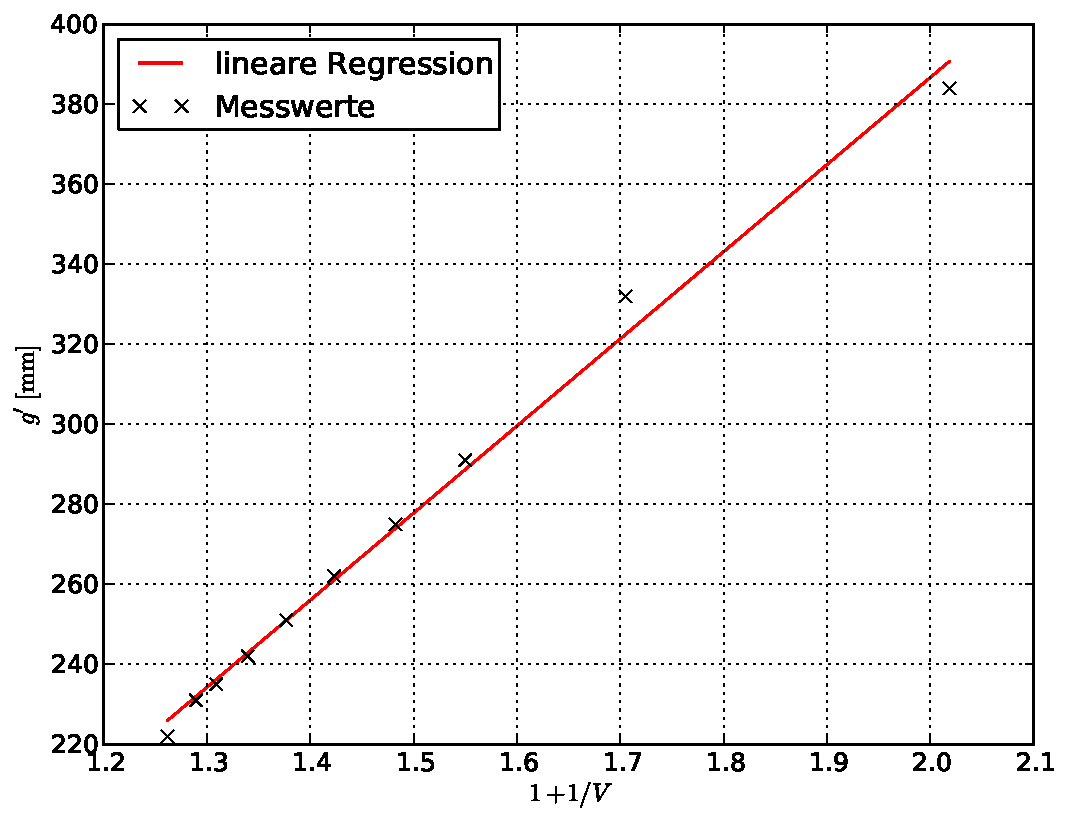
\includegraphics[width = 15cm]{img/graph_abbe_g.pdf}
			\caption{Lineare Regression $g'$ gegen $1 + 1/V$.}
			\label{fig:lin_reg_g}
		\end{figure}

		\begin{figure}[h!]
			\centering
			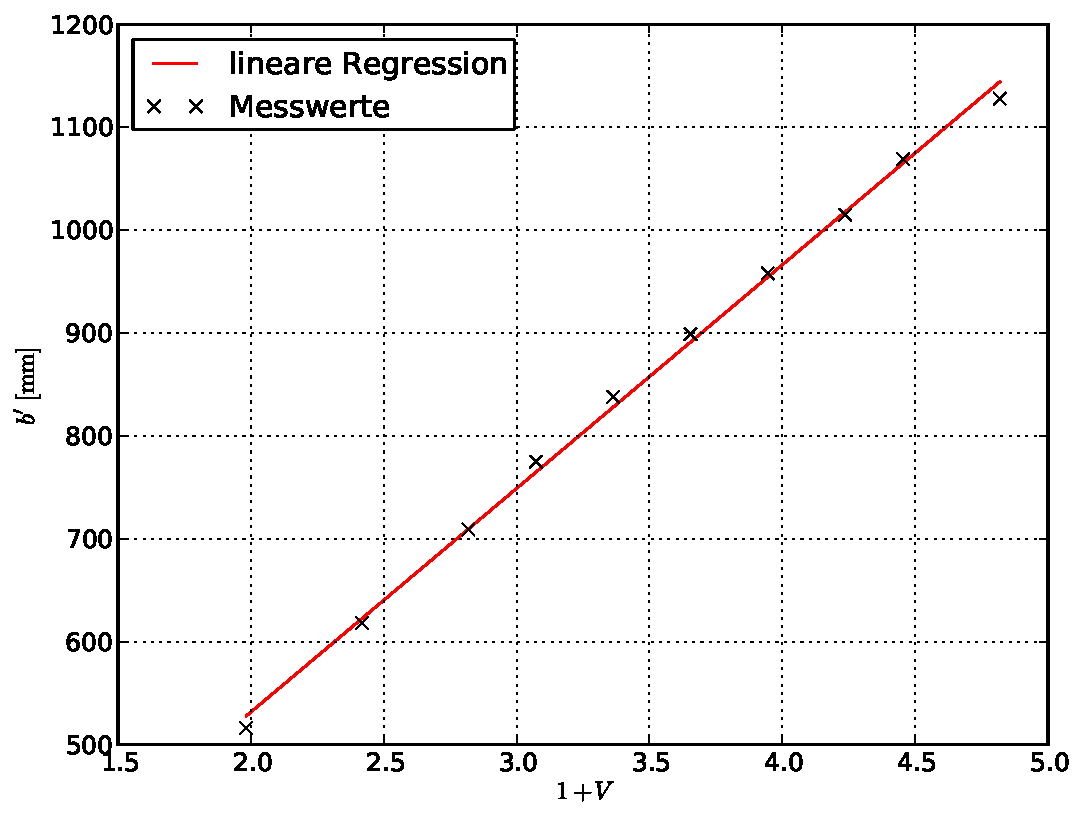
\includegraphics[width = 15cm]{img/graph_abbe_b.pdf}
			\caption{Lineare Regression $b'$ gegen $1 + V$.}
			\label{fig:lin_reg_g}
		\end{figure}